%%%%%%%%%%%%%%%%%%%%%%% file template.tex %%%%%%%%%%%%%%%%%%%%%%%%%
%
% This is a general template file for the LaTeX package SVJour3
% for Springer journals.          Springer Heidelberg 2010/09/16
%
% Copy it to a new file with a new name and use it as the basis
% for your article. Delete % signs as needed.
%
% This template includes a few options for different layouts and
% content for various journals. Please consult a previous issue of
% your journal as needed.
%
%%%%%%%%%%%%%%%%%%%%%%%%%%%%%%%%%%%%%%%%%%%%%%%%%%%%%%%%%%%%%%%%%%%
%
% First comes an example EPS file -- just ignore it and
% proceed on the \documentclass line
% your LaTeX will extract the file if required
%\begin{filecontents*}{example.eps}
%!PS-Adobe-3.0 EPSF-3.0
%%BoundingBox: 19 19 221 221
%%CreationDate: Mon Sep 29 1997
%%Creator: programmed by hand (JK)
%%EndComments
%gsave
%newpath
%  20 20 moveto
%  20 220 lineto
%  220 220 lineto
%  220 20 lineto
%closepath
%2 setlinewidth
%gsave
%  .4 setgray fill
%grestore
%stroke
%grestore
%\end{filecontents*}
%
\RequirePackage{fix-cm}
%
%\documentclass{svjour3}                     % onecolumn (standard format)
%\documentclass[smallcondensed]{svjour3}     % onecolumn (ditto)
\documentclass[smallextended]{svjour3}       % onecolumn (second format)
%\documentclass[twocolumn]{svjour3}          % twocolumn
%
\smartqed  % flush right qed marks, e.g. at end of proof
%
\usepackage{graphicx}
\usepackage{rotating}
\usepackage{url}
%
% \usepackage{mathptmx}      % use Times fonts if available on your TeX system
%
% insert here the call for the packages your document requires
%\usepackage{latexsym}
% etc.
%
% please place your own definitions here and don't use \def but
% \newcommand{}{}
%
% Insert the name of "your journal" with
% \journalname{myjournal}
%
\usepackage{afterpage}
\usepackage{csquotes}
\usepackage{lscape}
\begin{document}

\title{The Impact of Science Capital on Self-Concept in Science.}

%\thanks{Grants or other notes
%about the article that should go on the front page should be
%placed here. General acknowledgments should be placed at the end of the article.}

\subtitle{A Study of University Students in New Zealand}

%\titlerunning{Short form of title}        % if too long for running head

\author{Steven Martin Turnbull        %\and
       % Second Author %etc.
}

%\authorrunning{Short form of author list} % if too long for running head

\institute{S.M. Turnbull \at
              School of Critical Studies in Education, Faculty of Education and Social Work, The University of Auckland \\
              Tel.: +123-45-678910\\
              \email{s.turnbull@auckland.ac.nz}           %  \\
%             \emph{Present address:} of F. Author  %  if needed
           %\and
           %S. Author \at
        %      second address
}

\date{Received: date / Accepted: date}
% The correct dates will be entered by the editor


\maketitle

\begin{abstract}
Understanding factors that contribute to students' self-concept in science is an important task in boosting the number of students studying science and retaining students in science fields. A questionnaire was administered to science students at the University of Auckland (N = 693) to test a theoretical model of science self-concept tied to the work of Pierre Bourdieu. In this model, a student's social capital (i.e., relationships with parents, teachers and peers) and cultural capital (i.e., science related resources) are seen as key determinants of a student's belief that science is a domain in which they can succeed. Results from a simple Structural Equation Modelling (SEM) show that, of the factors included in the model, exposure to passionate science teachers during high school was the main predictor of self-concept for our sample of university science students. Implications of these findings are discussed in the context of the field of science education and Bourdieu's sociological theory.
\keywords{Science education \and Self-concept \and Social Capital \and Cultural Capital}
% \PACS{PACS code1 \and PACS code2 \and more}
% \subclass{MSC code1 \and MSC code2 \and more}
\end{abstract}

\section*{Introduction}
\label{intro}
Much research has been dedicated to understanding who chooses to study science at university, and what factors influence retention and completion of university science degrees. One particular factor that is associated with retention is students' confidence. Understanding students' confidence in science is important for several reasons. Students who are more confident in science are more likely to have better outcomes in science classes \cite{uccar2017role,tighezza2014modeling,chang2008science,peters2013examining} and hold aspirations for further study \cite{mujtaba2018students}, and graduate from university \cite{larson2015predicting}. In turn, graduating from university tends to lead to better life outcomes in general \cite{Oreopoulos_2007}, and greater economic outcomes \cite{norton2016mapping,mahoney2013moving}. Research on factors affecting student confidence also has important implications for government, as they seek skilled workers in STEM to help gain economic prosperity and growth \cite{pricewaterhousecoopers2015smart}. In New Zealand, the education system is not only charged with producing an increase in the number skilled workers in STEM domains, but producing confident learners. This message is made clear in the official high school curriculum:
\begin{quote}
   The New Zealand Curriculum is a clear statement of what we deem important in education. It takes as its starting point a vision of our young people as lifelong learners who are confident and creative, connected, and actively involved.
\end{quote} \cite{NZC}

A wealth of research has shown that disparities in tertiary science participation exist across the intersection of gender, ethnicity and social class \cite{reynolds2011change,meehan2017explaining}. Students from high Socio-Economic Status (SES) backgrounds are more likely to realise tertiary education goals \cite{reynolds2011change}, whilst interest in science also tends to differ across SES, gender \cite{cheryan2017some}, and ethnicity \cite{Wong2016ScienceStudents}. Previous theorists have used metaphors, such as the \textit{gender filter} \cite{Blickenstaff_2005} and the \textit{smog of bias} \cite{Kost_Smith_2010} that consider the way contextual factors impact on student outcomes. For example \cite{Kost_Smith_2010} argues that gender disparities can not be attributed to one specific factor, but instead there are a range of factors and small effect sizes that contribute to inequity. Confidence is often cited as a reason for why we see disparities in participation and retention across social groups, particularly in STEM \cite{Blickenstaff_2005}.  

However, a student's confidence does not exist in a vacuum. It is important to consider the factors that relate to confidence in STEM domains. Why does gender, ethnicity, and social class often share a relationship with students' confidence? The goal of this article is to explore the factors affecting confidence further, using a theoretical framework that can answer this question. More specifically, we hope to highlight the way in which confidence is rooted in societal structures. To do this, we employ the sociological theory of Pierre Bourdieu. Recent research has made use of Bourdieu's sociological theory as a framework for understanding the uneven patterns in student interests and pursuits \cite{archer2013aspires,Archer_2015}. Bourdieu's theory enables us as researchers to place individuals in the context of their environment, and to understand the how social, cultural, and historical factors structure the world in which individuals live, and the internal dispositions they hold. The following section will outline Bourdieu's theory in more detail, with specific reference to \textit{science capital}. As summarised by Archer et al., \cite{Archer_2015} science capital is a concept that facilitates the application of a Bourdiusian framework to research on science education. It will provide an introduction to Bourdieu's theory, and outline the concept of science capital in more detail. It will define the component parts of economic, cultural, and social capital, and detail the utility of the concept in placing student outcomes in a broad, complex, theoretical framework. We follow this section by discussing the link between self-concept and Bourdieu's theory through the concept of habitus.

\subsection*{Bourdieu and Science Capital}
\label{sciencecapital}
Capital can be defined as the resources that one can use to gain advantage in society \cite{Bourdieu_1986}. According to Bourdieu, capital can take various forms. These include economic, cultural, and social. Economic capital refers to an individual's financial resources (e.g., money, investments). cultural capital refers to an individual's non-financial resources, such as the object they own (e.g., books, clothing, furniture), or the characteristics they embody (e.g., accent, posture). Bourdieu defines social capital as the economic and cultural capital that we are able to generate through our relationships with other individuals. With all forms of capital, the value is determined by the \textit{field} in which it is being used. To give a basic example, owning science books may be of value for someone studying in the field of science, but this is of less value to someone studying opera. The current study focuses on the field of science, and the forms of capital that have been found to impact on outcomes in science. Contemporary research has applied Bourdieu's sociology to understand why students choose to study science, with the concept of Science Capital \cite{Archer_2015}. Science capital has been described by \cite{Archer2014} as a:
\begin{quote}
conceptual device for collating various types of economic, social and cultural capital that specifically relate to science --- notably those which have the potential to generate use or exchange value for individuals or groups to support and enhance their attainment, engagement and/or participation in science.
\end{quote}
These economic, social and cultural factors are important to consider when exploring student outcomes in science. 

\subsection*{Economic Capital}
Simply put, the concept of economic capital refers to an individuals' financially assets (e.g., money). The benefits of economic capital are well studied and relatively easy to interpret. Research from international studies such as TIMSS have shown that higher SES is linked to better student outcomes during high school \cite{Mullis_2012,mullis2016timss}, and this trend does apply to students in New Zealand specifically \cite{May_2016}. As outlined by Bourdieu \cite{Bourdieu_1986}, the value of economic capital comes from its exchange value. For example, students with from economically wealthy families are likely able to afford books, laptops, and other aids to study. In paying for these objects, students are exchanging economic capital for non-financial assets. Bourdieu categorizes these non-financial assets under the term cultural capital, and it is through cultural capital that educational advantages are accumulated. Recognising the role of non-financial forms of capital, and with it the social relationships that facilitate access to capital, is complex. In doing so, however, we are able to develop a theoretical model of social class that takes into account factors beyond economic wealth. 

\subsubsection*{Cultural Capital}
Cultural capital refers to the non-financial resources an individual has at their disposal \cite{Bourdieu_1986}. Cultural capital is a complex concept as it is manifested in the objects that one owns (e.g., books, furniture, clothing), or embodied (e.g., in our posture, accent, bodily physique). With regards to science, cultural capital may take the form of objects that are used in, such as chemistry sets, laptops, or books. Students may also boost their cultural capital in science with access to other science-related resources, such as visiting science museums \cite{Dawson2014} or after-school science clubs \cite{mujtaba2018students}. Cultural capital can play an important role in students' progression to university study \cite{aschaffenburg1997cultural}. This is echoed in the field of science education, where research has found that access to science related cultural capital is associated with decisions to study science further in high school \cite{mujtaba2018students}, and at university \cite{Lyons_2006}.

The manner in which students embody their cultural capital may also carry different value in science. Research has found that scientists are typically viewed as old, white males \cite{Nosek_2009,Barthelemy_2016}, and that individuals who differ from this stereotype may face barriers to acceptance in the field \cite{ong2005body}. Research has shown that women tend to be viewed as less competent in science solely in terms of their gender in many different roles, whether the it involves a student, applications to a lab assistant role \cite{Moss_2012}, or quality assessment of science teachers \cite{Potvin_2016}. 

\subsubsection*{Social Capital}
Having social relationships with individuals who hold valuable forms of capital is highly beneficial. For example, for a student studying at university, having parents who also studied at university may lead to better outcomes. These students are not only more likely to have access to educational resources (objectified cultural capital), but they may also be exposed from an early age to an academic way of life (embodied cultural capital).

One of the most important social relationships for students is their relationship with their teachers. Teachers play an integral role to students' experiences within the field of education. The content knowledge that teachers hold can be an important form of social capital for students \cite{goldhaber2000does,wayne2003teacher,keller2017impact}, while the attitudes and behaviours of teachers can significantly impact on the interest students hold in STEM \cite{keller2017impact} and the level of confidence students have in themselves. As outlined by researchers such as \cite{bandura1986explanatory} and \cite{siegle2007increasing}, STEM teachers can boost the self-concept of their students by encouraging students and recognising their ability. For example, students' who feel recognised as being good at physics are more likely to hold further interest in physics \cite{Hazari2017}. Through a Bourdieusian lens, recognition provides a signal to students that the field is somewhere they belong. Studies of classroom environments have continuously shown that positive teacher-student interactions are a strong source of interest in science \cite{osborne2003attitudes,keller2017impact}. \cite{mujtaba2018students} found that encouragement was an especially important influence in students aspirations to study chemistry. The social capital provided by teachers may be particularly important for students choosing to study in fields where they are members of an underrepresented group, or where their capital is undervalued by those with power in the field.

It is also important to consider the impact of students' social relationships with their peers in science outcomes \cite{osborne2003attitudes}. Adolescence is a time where individuals begin to be increasingly influenced by their peers \cite{douvan1966adolescent}, which can impact on academic engagement and achievement \cite{ryan2000peer}. Students may be subjected to group norms that may influence the decisions they make with regards to future study \cite{brown1986perceptions}. Following this, it is no surprise that individuals belonging to friendship groups that value science may be more likely to have motivations to pursue science further \cite{robnett2013friendship}. Other research shows that students' persistence in STEM domains at university may be influenced by their academic peer groups \cite{Ost_2010}.

Finally, students' social capital is bolstered by their relationships within the family. Parents' educational expectations for their children is a key predictor of educational aspirations \cite{wu2015early}. In science \cite{Lyons_2006} found that parents' attitudes towards educational qualifications and encouragement were important factors relating to students' decisions to study science. Students with highly educated parents are also much more likely to fulfil goals of attaining tertiary qualifications \cite{reynolds2011change}, while students with parents who are employed in STEM occupations are more likely to choose to major in STEM at university \cite{moakler2014college}. These findings point to Bourdieu's concept of social reproduction, where the social position of families are transferred across generations. Parents who are university educated may be more likely to engage in concerted cultivation - the process of deliberately building children's cultural capital \cite{lareau2011unequal}. Parents from higher SES backgrounds may hold higher educational expectations for their children \cite{carolan2015does}, whilst they may also be more involved in their children's education \cite{cheadle2011quantitative}. Beyond the deliberate cultivation of their children, parents who studied science at university are also more able to use science-related discourse which is an important manifestation of cultural capital \cite{Lyons_2006,bernstein1971class}. The role of the family goes beyond typical forms of social capital, as the family provides the context in which individuals develop their identity. For this reason, we relate family-related factors to Bourdieu's concept of habitus. 

\subsubsection*{Habitus}
As previously discussed, students experiences within fields and their interactions with resources may begin to be embodied physically as embodied cultural capital. At the same time, students also embody these experiences \textit{mentally}. The mental embodiment of capital can be summarised by Bourdieu's concept  of \textit{habitus}. Bourdieu defines habitus as the internal dispositions that an individual holds that generate practices within the field. While an individual's volume of capital may determine their position in the field, their habitus determines their disposition towards the field \cite{bourdieu1992invitation}. Habitus represents an individuals internalisation of society --- the resulting mental structure of the process commonly referred to as socialisation \cite{Nash1999}.

For Bourdieu, habitus is the mechanism which mediates between structure and agency. Students internalise the environment in which they are placed and make judgements on what is possible and realistic ``for them''. A student's family background is likely to have a integral role in shaping habitus. Students from families that are familiar with university or have a history of working in science related fields may be more likely to have internalised dispositions that see science as something that is for them. A student's habitus is influenced by their familial context \cite{Dimaggio1982}, with some theorists pointing to the concept of ``family habitus'' as a tool to understand how family resources, values, and life style choices are internalised by children \cite{Archer2012,tomanovic2004family}. The resources available to students through their family are thus extremely important, not only because they offer objectified forms of cultural capital, but also because they offer exposure to ways of thinking and understanding that have been proven to be valued by educational institutions. Students may be more likely to view science as a realistic study choice, and university as a possible destination, if they have parents who have modelled these trajectories previously \cite{Lyons_2006}. 

Much research has discussed applications of habitus in education research \cite{Reay_2004,Nash1999}, although the concept is often criticised for being too complex \cite{goldhaber2000does} and difficult to operationalise \cite{dumais2002cultural}. Most research on habitus has been qualitative, but, as outlined by \cite{mu2014heritage}, there is an increasing need to consider quantitative applications of habitus. The current study seeks to operationalise habitus quantitatively by through the use of a simple science self-concept inventory. The construct of science self-concept was chosen as it relevant for university science students and can be theoretically tied to arguments outlined by Bourdieu regarding habitus \cite{mu2014heritage,bodovski2014adolescents}. The following sections will describe self-concept in more detail and explain it's relevance to Bourdieu's theory and the current study.   

\subsection*{Self-concept}
\label{selfconcept}
While quantitative applications of habitus in education research are relatively rare, quantitative applications of self-concept have been more widely used, operationalised and validated \cite{marsh2014academic,hattie2014self}. Self-concept can be defined as the way in which an individual perceives their self \cite{rosenberg1979conceiving,shavelson1976self} and is influenced by environmental sources located outside of the individual, such as the appraisals of others. As outlined by \cite[p.488]{shavelson1976self} ``Self-concept may be described as: organized, multifaceted, hierarchical, stable, developmental,
evaluative, and differentiable.'' Self-concept is therefore not too theoretically dissimilar from habitus, which has been defined as a ``system of dispositions'' [p.471] that is multifaceted \cite{Nash1999}, and ``durable but not eternal'' \cite{Bourdieu1984}. Scores on inventories assessing self-concept can thus be interpreted through the lens of Bourdieu in a productive manner, with this being evidenced in prior research \cite{dumais2002cultural}.  Importantly, the decision to interpret self-concept in terms of student habitus is necessary as it: ``ensures that the research focus is always broader than the specific focus under study'' \cite{Reay_2004}. In other words, using the concept of habitus facilitates the understanding of how an individual's self-concept is generated in relation to the socio-cultural context in which an individual lives. Given the similarities between self-concept and habitus, self-concept inventories are an appropriate and useful tool to explore an individual's habitus. As described by \cite[p.395]{bodovski2014adolescents}, we may view both general and area-specific self-concepts as ``illustrations of different aspects of habitus.''  

Few New Zealand based studies have explored university students' motivations, dispositions or self-belief in science. In one such study, Dalgety and Coll (2006) \cite{dalgety2006exploring} explored the self-efficacy of first year university chemistry students in New Zealand across three time points in an academic year. They detailed gender differences in specific items related to self-efficacy, finding that male students tended to report higher scores (for example in their belief that they could achieving a passing grade in a chemical hazards course). While the work of Dalgety and Coll offers many insights into self-efficacy at university in the context of New Zealand, the lack of research in this area, especially within the last decade, is a lacuna to be filled. 


\subsection*{The Current Study}
\label{sec:3}

The current study seeks to address these two gaps in the research by exploring the impact of science capital on self-concept in science for university students in New Zealand. More specifically, we apply Pierre Bourdieu's \cite{Bourdieu_1986,Bourdieu1984} concepts of capital and habitus to explore the interaction between students' access to resources and internal dispositions. Whilst the factors affecting outcomes in science are wide-ranging 
\cite{osborne2003attitudes}, we focus on the impact of science-related resources and social experiences in science on student's self-concept in science. In doing so, we are able to assess the impact of social class on self-concept, but using a definition of class defined in terms of \textit{capital} (social, cultural, and economic wealth), as opposed to solely economic wealth. Our specific hypotheses are as follows. We expect:
\begin{itemize}
    \item Higher levels of science-related social and cultural capital to be associated with higher levels of self-concept in science. 
    \item Relationships with high school teachers will be the most important form of social capital. This is based on the idea that teachers are experts in the field and their judgements provide the most domain-specific feedback. In terms of habitus, students will be more likely to internalise the idea that they are good at science if they have an expert (the teacher) encourage them and/or recognise their ability. 
    \item Male students will have higher levels of self-concept than female students. This is based on previous research that has identified gender disparities in confidence in science \cite{Ellis_2016}. 
    \item The number of university generations within the students family, and having parents positively orientated towards science will be positively associated with self-concept. We would expect students who have available academic role models in their family to have a habitus that is predisposed to university science study. They will likely be more likely to engender the belief that university is somewhere where they belong, and somewhere that they can be successful, because that is what their family does. 
\end{itemize}
While acknowledging that differences in science self-concept may exist across ethnic groups, the decision was made to exclude this from our analysis. This is due to several reasons. Firstly, we seek to follow kaupapa M\={a}ori values. This means that research concerning M\={a}ori should be done by M\={a}ori and for the benefit of M\={a}ori. \cite{walker2006exploration} The current study seeks to benefit M\={a}ori by providing a step towards understanding the factors impacting on science self-concept which may inform future research in this area. Secondly, our conceptual model is theoretically grounded in western ways of thinking and knowing about science and culture. More work is needed to consider ways of knowing and constructing science and culture that are grounded in M\={a}ori ways of knowing, such as M\={a}tauranga. \cite{hikuroa2017matauranga} We hope that the results of the current study can aid in this endeavour. 
\begin{figure*}
 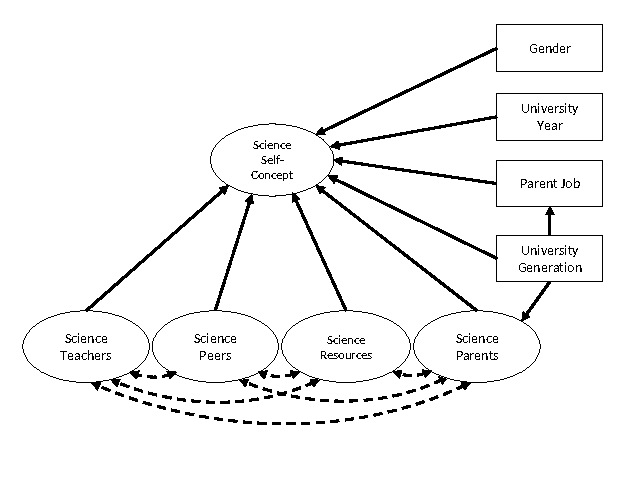
\includegraphics{ConceptualModel.eps}
\caption{Conceptual Model. Latent variables are represented by oval boxes, observed variables are represented by rectangular boxes. Regressions are represented by one-sided arrows, while correlations are represented by double headed arrows and dashed lines. }
\label{fig:1}       
\end{figure*}

\section*{Methodology}
\label{method}
\subsection*{Data}
\label{data}
During the first semester of 2019, an online questionnaire was administered to science students at the UoA via email. In order to boost the rate of response, the questionnaire was designed to be quick (10 minutes), consisting of 48 items. Questionnaire responses were anonymous, with the exception of students who left their email to be entered into a prize draw. In total, 693 students completed the questionnaire (the sample is summarised in Table \ref{tab:Sample}. 


\begin{table}[h]
\centering

\label{tab:Sample}       % Give a unique label
\begin{tabular}{lccc}
\hline
                                                             & N   & Mean & SD   \\ \hline
Male                                                         & 685 & 0.36 & 0.48 \\
Female                                                       & 685 & 0.63 & 0.48 \\
Gender Diverse                                               & 685 & 0.01 & 0.08 \\
Euro                                                         & 693 & 0.53 & 0.5  \\
Asian                                                        & 693 & 0.44 & 0.5  \\
Pasifika                                                      & 693 & 0.04 & 0.2  \\
M\={a}ori                                                        & 693 & 0.07 & 0.26 \\
MELAA*                                                        & 693 & 0.03 & 0.18 \\
Other Ethnicity                                               & 693 & 0    & 0.07 \\
Parent Job  (0-4) & 681 & 2.61 & 0.71 \\
Uni generations (0-3)                                        & 687 & 1.67 & 1.04 \\ \hline
\end{tabular}
\caption{Sample description. Counts, means and standard deviations (SD) of sample characteristics. All items recorded on a binary scale (1 indicating category applies), unless otherwise specified. *Middle Eastern, Latin American, or African} 
\end{table}

The questionnaire asked students for factual information about themselves, and also questions regarding 5 latent constructs informed and adapted from the work of \cite{dewitt2011high}. The constructs, outlined in our conceptual model (see Figure 1), included self-concept in science (Science Self-concept), experience of high school science teacher quality (Science Teachers), parental attitudes towards science (Science Parents), peer attitudes towards science (Science Peers), and access science-related resources (Science Resources). The first 4 constructs were measured through items asking students to rate their agreement regarding a statement on a continuous scale from 0 to 100. The continuous scale was favoured over more traditional likert scales given the bias of the sample. As students in our sample have all chosen to pursue science at university, most students will likely score highly on these items. The continuous scale, in addition to being easier for participants in practice, allows for increased variance in scores. The final construct, access to Science Resources, was measured on a 1-5 scale, where students were asked how often they participated in a science related activity (1 being never, 5 being once a week). For all constructs, item statements and loadings can be seen in Table \ref{tab:ItemMeansSDs}. Other questions asked for factual information, such as gender, ethnicity, family’ education, and parents' job. 

The following variables were included in our analyses:
\begin{itemize}
    \item \textbf{Science Self-concept}. We use items from the positive and negative self-concept scales of \cite{dewitt2011high} (``I am good at science'', ``If I study hard I will do well in science courses''.   
    \item \textbf{Science Teachers}. Experience of high school science teachers refers to the extent to which students recall having positive experiences with their high school science teachers. This scale refers to the degree of enthusiasm, care and recognition the student perceived. 
    \item \textbf{Science Parents}. Parental attitudes towards science was adapted from the Parental attitudes towards science scale of \cite{dewitt2011high}. The item ``My parents would be happy if I became a scientist when I grow up'' was replaced with ``My parents/carers would like it if I worked in science'' to better reflect the target population.
    \item \textbf{Science Peers}. Peer value of science was measured through items adapted from the ``Peer orientation towards school'' and ``Peer attitudes towards science'' scales of \cite{dewitt2011high}. One item, Q4.1 (``My friends see me as a `science' person''), did not load on to the construct. It is likely that this construct represents the participants view of their peers, as opposed to the students' subjective experience of their peers perception of them.
    \item \textbf{Science Resources}. Student's access to resources was adapted from \cite{dewitt2011high}. To suit our target audience, we replace the original phrase ``How often do you do the following things when you are NOT in school...'', with ``Growing up, how often did you...''. One item, Q5.5 (``Growing up, did you go to a lunchtime or after-school science club?'') did not load onto the construct. This may be due to the low number of students who responded positively to this question. An important point to consider is that we, as researchers, are defining science-related cultural capital in our own terms. Whilst the items used in the current study are by definition forms of capital, we acknowledge that other forms of capital exist and hold value in different socio-cultural contexts.
    \item \textbf{University Generations}. University Generations is a count score of the number of consecutive generations a participants family has gone to university. First generation students receive a score of 0,  participants who had siblings attend receive a score of 1, participants who had parents attend university receive a score of 2, and those who had parents and grandparents attend receive a score of 3.
    \item \textbf{Parents Job}. Participants were asked to state the profession of their father/male carer and their mother/female carer. The professions were classified according to the Australian and New Zealand Standard Classification of Occupations (ANZSCO), where a score of 0 is unemployed, 1 is low skilled, and 4 is highly skilled. The Parents Job score is the maximum value of both parents scores.
    \item \textbf{Gender}. Gender was recorded using an open text box, and then categorised according to the classification set out by Statistics New Zealand. Of the 693 students who completed the survey, only 1\% did not record a gender. 

\end{itemize}

\begin{landscape}
\begin{table}[ht]
\label{tab:ItemMeansSDs}       % Give a unique label

\centering
\begin{tabular}[width = \textwidth]{clclccccc}
  \hline
Item Code & Item Statement & Loading & Construct & N & Mean & SD & Skewness & Kurtois \\
  \hline
Q1.1 & I understand everything in my science courses & 0.62 & Science Self-concept & 617 &68.75 & 19.73& -0.94&0.78\\
Q1.2 &   I find science difficult & -0.40 & Science Self-concept & 606 & 50.19 & 24.68 & -0.02&-0.78\\
Q1.3 &   I get good marks in science tests & 0.72 & Science Self-concept &617 & 67.50&18.06 & -0.42&0.06\\
Q1.4 &  If I study hard, I will do well in my science courses & 0.54 & Science Self-concept &620&86.69 &14.85	 &-1.59&3.53\\
Q1.5 &  I am just not good at science & -0.38 & Science Self-concept & 605& 20.41& 19.28& 0.85&-0.07\\
  \hline
Q2.1 &  My high school teachers recognised that I was good & 0.75 & Science Teachers &615&69.08	 &19.10 & -0.80&-0.28\\
&at science&&&&&&&\\
Q2.2 &  My high school teachers cared whether I understood& 0.72 & Science Teachers &618&70.61 &26.34 & -0.88&0.01\\
&science&&&&&&&\\
Q2.3 &  My high school teachers explained to me that science& 0.64 & Science Teachers &615&65.24&27.05 &-0.56	&-0.55	\\
& is useful for my future&&&&&&& \\
Q2.4 &   My high school science teachers were enthusiastic & 0.64 & Science Teachers &619	&75.74&23.70 & -1.06&0.52	\\
&about science&&&&&&& \\
Q2.5 &  My teachers have specifically encouraged me to continue & 0.74 & Science Teachers &593&52.78&32.75 & -0.10&-1.23\\
& with science after school&&&&&&& \\
  \hline
Q3.1 & My parents/carers think science is interesting & 0.59 & Science Parents &618	&70.62&	23.64	 &-0.75	&0.14  \\
Q3.2 & My parents/carers think it is important for me to learn science & 0.88 & Science Parents &619&65.73&26.46	 &-0.48	&-0.54	\\  
Q3.3 & My parents/carers would like it if I worked in science & 0.77 & Science Parents   &612&66.06&27.28 & -0.56&-0.45\\
Q3.4 & My parents/carers have explained to me that science is & 0.80 & Science Parents & 592	&53.65	&31.64	& -0.10	&-1.16	\\  
&useful for my future&&&&&&&\\
  \hline
Q4.1 & My friends see me as a ``science person'' & - & - &  602	&70.23&	28.11 &-0.86&-0.14\\
Q4.2 & My friends think that science is important & 0.91 & Science Peers & 615&68.61&	23.47 & -0.65&-0.03 \\
Q4.3 & My friends think science is cool & 0.83 & Science Peers &617&63.38&25.90 & -0.44&-0.48\\ 
Q4.4 & My friends care about their university grades & 0.40 & Science Peers &619&	81.10&	21.21 &-1.56&2.65 \\
  \hline
Q5.1 & Growing up, did you do science activities (e.g.,  & 0.55 & Science Resources& 581	&2.40&0.87 & 0.09&-0.68 \\ 
&science kits, nature walks, do experiments)?&&&&&&&\\
Q5.2 & Growing up, did you read books or magazines about & 0.69 & Science Resources &572	&2.42&1.01 & 0.03&-1.11\\
&science?&&&&&&&\\
Q5.3 & Growing up, did you look up things online about science & 0.69 & Science Resources &592&2.97&0.97 &-0.54&-0.79	\\
&or nature?&&&&&&&\\
Q5.4 & Growing up, did you watch TV programmes about science & 0.62 & Science Resources &599&2.89&0.91 &-0.43&	-0.64\\
&or nature?&&&&&&&\\
Q5.5 & Growing up, did you go to a lunchtime or after-school & - &-&579&1.50&0.93 & 1.65&	1.30\\
&science club?&&&&&&&\\

   \hline
\end{tabular}
\caption{Questionnaire Items. Table showing the questionnaire items used in the current study, with loadings onto the relevant latent construct where applicable. Descriptive statistics for each item are also reported. All items were scored on a continuous scale of 0-100, with the exception of Q5 items, which were scored on a likert scale of 1-5.} 
\end{table}
\end{landscape}

Multiple imputation was used to avoid list wise deletion of cases with missing data, as we cannot make the assumption that data is missing completely at random. Missing data for the construct items were imputed using Predictive Mean Matching (PMM). Cases that were missing scores on at least half the items from a construct (37 cases) were excluded from analysis (e.g., with a construct with 5 items, cases missing scores on 2 items would be kept, whilst cases missing scores on 3 or more items would be excluded). Mature students (those with a recorded age over 24) were also excluded (42 cases). A further 31 students were excluded from analysis due missing data on non-imputable variables, such as parents job, university generations, or gender. Imputation allowed us to retain 174 cases that would otherwise be excluded with list wise deletion, leaving a  sample size of 583 students. Whilst the questionnaire items are adapted from previous work, exploratory factor analysis (EFA) and confirmatory factor analysis (CFA) were carried out to test the validity of our latent constructs. Concurrent and convergent validity \cite{campbell1959convergent} of these measures were then established through EFA and CFA, and found to be at an adequate level. We used Cronbach's $\alpha$ and McDonald's $\omega$ to test internal consistency, with both providing similar reliability scores. McDonald's $\omega$ and Cronbach's $\alpha$ were fine for all constructs ($\alpha$ ranging from 0.75 to 0.85), except Self-concept which had an $\alpha$ of 0.68. Whilst 0.70 is usually considered an acceptable level for internal consistency, it has been argued that $\alpha$ below 0.70 are not uncommon for attitudinal scales \cite{field2012discovering}. 

\subsection*{Structural Equation Modelling}
Structural Equation Modelling (SEM) was used to analyse the conceptual model outlined in Figure 1. SEM comprises two parts, the measurement model and the structural model. The measurement model shows the loadings of manifest variables onto each latent construct, while the structural model shows the interrelations between the latent constructs and other variables in the conceptual model \cite{schreiber2006reporting}. In our model, Science Self-concept is viewed as a dependant variable, predicted by Science Teachers, Science Peers, Science Parents, and Science Resources. We also include other manifest variables as predictors, including Gender, University Generations, University Years, and Parent Job. We also model correlations between our latent constructs, and University Generations is modelled as a predictor of Science Parents and Parent Job.

SEM with robust standard errors \cite{huber1967behavior,white1982maximum} was carried out on 5 imputed datasets using the Lavaan \cite{rosseel2012lavaan} and semTools \cite{jorgensen2018package} packages in R \cite{team2013r}. Rubin's rules \cite{rubin2004multiple} were used to pool point and standard error estimates across our imputed data sets. 


\section*{Results}
\label{results}
Descriptive statistics, including means and standard deviations are summarised in Table \ref{tab:ItemMeansSDs}. Correlations between constructs, shown in Table \ref{tab:Correlations}, show that Science Self-concept is positively correlated with each form of science capital explored in the current study. Science Self-concept was most positively associated with Science Teachers ($r = 0.35$), and most weakly correlated with Science Resources ($r = 0.16$). We now detail the results of the SEM which explores the relationships between these constructs while including other factors present in the theoretical model (Figure \ref{fig:1}).

\begin{table}[ht]
\label{tab:Correlations}       % Give a unique label
\begin{tabular}{lccccc}
\cline{2-6}
                  & Science Self-concept & Science Teachers & Science Parents & Science Peers & Science Resources \\ \hline
Science Self-concept  & 1                & -                & -               & -             & -                 \\
Science Teachers  & 0.35            & 1                & -               & -             & -                 \\
Science Parents   & 0.21            & 0.31            & 1               & -             & -                 \\
Science Peers     & 0.26            & 0.30            & 0.49            & 1             & -                 \\
Science Resources & 0.16            & 0.19            & 0.28           & 0.35         & 1                 \\ \hline
\end{tabular}
\caption{\textbf{Correlations between constructs for CFA}  Variables were standardized to have a mean of 0 and a standard deviation of 1. CFA =
confirmatory factor analysis. N = 583; M = 0; SD = 1.}
\end{table}

We performed a SEM analysis with robust standard errors to test the conceptual model shown in Fig \ref{fig:1} on a sample of 583 undergraduate science students. A correlation table with means and standard deviations is shown in Table \ref{tab:Correlations}. While the hypothesized model appears to be a okay fit to the data (CFI = .904; TLI = .885;  RMSEA = .053, gamma hat =  .928), model fit was improved with the inclusion of two modifications. Specifically, we added two additional correlations between items Q2.1 and Q2.3, and items Q2.2 and Q2.4. With these modifications, goodness of fit statistics showed acceptable model fit \cite{hu1999cutoff,steiger2007understanding} ($\chi$ = 598.38, df = 258, Gamma hat = 0.95, CFI = 0.93, TLI = 0.91, RMSEA = 0.05, SMSR = 0.05). As shown in Table \ref{tab:MeasurementModel}, the standardized loadings were all significant and acceptable. 



\begin{table}[ht]
\label{tab:MeasurementModel}       % Give a unique label
\centering
\begin{tabular}{llrrrrr}
  \hline
Latent & Manifest & Estimate & StandardError & z & p & Standardized \\ 
  \hline
Science Self-concept & Q1.1 & 1.00 &  &  &  & 0.65 \\ 
   & Q1.2 & -0.80 & 0.11 & -6.99 & $<$ .01 & -0.43 \\ 
   & Q1.3 & 1.03 & 0.09 & 11.00 & $<$ .01 & 0.72 \\ 
   & Q1.4 & 0.61 & 0.07 & 8.80 & $<$ .01 & 0.55 \\ 
   & Q1.5 & -0.60 & 0.08 & -7.70 & $<$ .01 & -0.39 \\ 
  Science Teachers & Q2.1 & 1.00 &  &  &  & 0.75 \\ 
   & Q2.2 & 0.94 & 0.06 & 14.65 & $<$ .01 & 0.70 \\ 
   & Q2.3 & 0.97 & 0.08 & 12.80 & $<$ .01 & 0.72 \\ 
   & Q2.4 & 0.75 & 0.07 & 11.03 & $<$ .01 & 0.62 \\ 
   & Q2.5 & 1.18 & 0.08 & 14.51 & $<$ .01 & 0.74 \\ 
  Science Parents & Q3.1 & 1.00 &  &  &  & 0.59 \\ 
   & Q3.2 & 1.65 & 0.12 & 14.05 & $<$ .01 & 0.88 \\ 
   & Q3.3 & 1.51 & 0.13 & 12.06 & $<$ .01 & 0.77 \\ 
   & Q3.4 & 1.81 & 0.14 & 12.82 & $<$ .01 & 0.82 \\ 
  Science Peers & Q4.2 & 1.00 &  &  &  & 0.93 \\ 
   & Q4.3 & 0.99 & 0.06 & 16.26 & $<$ .01 & 0.82 \\ 
   & Q4.4 & 0.39 & 0.05 & 7.82 & $<$ .01 & 0.41 \\ 
  Science Resources & Q5.1 & 1.00 &  &  &  & 0.56 \\ 
   & Q5.2 & 1.43 & 0.11 & 12.69 & $<$ .01 & 0.69 \\ 
   & Q5.3 & 1.40 & 0.15 & 9.18 & $<$ .01 & 0.69 \\ 
   & Q5.4 & 1.16 & 0.13 & 8.84 & $<$ .01 & 0.63 \\ 
   \hline
\end{tabular}
\caption{\textbf{Measurement Model}. The measurement model summarises the loading of items onto theoretical constructs outlined in Figure \ref{fig:1}. The results of the measurement model show that items loadings were significant and acceptable} 

\end{table}

The structural model, shown in Table \ref{tab:StructuralModel}, shows the interrelationships of the latent variables (specifically the impact of constructs on Science Self-concept) and the other observed variables in our conceptual model. 

\begin{table}[ht]
\caption{Structural Model} 

\centering
\begin{tabular}{llrrrrr}
  \hline
 Regressions &  & Estimate & Standard Error & z & p & Standardized \\ 
  \hline

  Science Self-concept & Science Teachers & 0.21 & 0.04 & 5.78 & $<$ .01 & 0.33 \\ 
   & Science Parents & -0.02 & 0.06 & -0.42 & .68 & -0.03 \\ 
   & Science Peers & 0.10 & 0.04 & 2.66 & $<$ .01 & 0.16 \\ 
   & Science Resources & -0.04 & 0.18 & -0.22 & .82 & -0.02 \\ 
   & Parent Job & 0.13 & 0.10 & 1.23 & 0.22 & 0.07 \\ 
   & Uni generations & 0.15 & 0.07 & 2.3 & 0.02 & 0.12 \\ 
   & Male & 0.46 & 0.12 & 3.67 & $<$ .01 & 0.17 \\ 
   & Uni Years & -0.13 & 0.06 & -2.28 & 0.02 & -0.10 \\ 
  Science Parents & Uni generations & 0.25 & 0.06 & 4.10 & $<$ .01 & 0.19 \\ 
  Parent Job & Uni generations & 0.21 & 0.03 & 7.14 & $<$ .01 & 0.32 \\ 
  \hline
Covariances &  &  &  &  & &  \\ 
  \hline
  Science Parents & Science Peers & 1.42 & 0.19 & 7.4 & $<$ .01 & 0.48 \\ 
  Science Teachers & Science Parents & 0.96 & 0.16 & 6.02 & $<$ .01 & 0.35 \\ 
  Science Parents & Science Resources & 0.17 & 0.04 & 4.00 & $<$ .01 & 0.25 \\ 
  Science Teachers & Science Peers & 1.35 & 0.23 & 5.90 & $<$ .01 & 0.31 \\ 
  Science Peers & Science Resources & 0.37 & 0.06 & 5.82 & $<$ .01 & 0.35 \\ 
  Science Teachers & Science Resources & 0.19 & 0.06 & 3.40 & $<$ .01 & 0.20 \\ 
   
   \hline
\end{tabular}
\label{tab:StructuralModel}
\caption{\textbf{Structural Model}. The structural model summarises the inter-relationships between the constructs identified in the measurement model (Table \ref{tab:MeasurementModel}) and the other variables included in the theoretical model (Figure  \ref{fig:1}). The results of the structural model show that while all of the science capital related constructs (Science Teachers, Science Peers, and Science Resources) are positively and significantly correlated, Science Teachers and Science Peers were the only significant predictors of Science Self-concept. Of the other variables included in the model, the number of university generations in the family (Uni Generations) and being male (Male) positively and significantly predicted Science Self-concept. The number of years a student had attended university negatively and significantly predicted Science Self-concept.} 
\end{table}

Results of the structural model show that Science Teachers had the most impact on students' Science Self-concept with a significant standardised estimate of 0.33. Of the other science capital related constructs, Science Peers was the only other significant predictor of Science Self-concept (0.16). For the other predictors in our model, the number of university generations in the family (Uni Generations) and being male positively predicted Science Self-concept (standardised estimates of 0.12 and 0.17 respectively). The number of years a student reported being at university (Uni Years) was a significant negative predictor of Science Self-Concept (-0.10). 

\section*{Discussion}
\label{discussion}
Our results show that, while social capital and cultural capital in science are all positively associated with the science self-concept of university science students, the social relationships shared with teachers and peers are the most important. For university science students, parent's value of science and the science related resources students had growing up were relatively insignificant predictors of science self-concept. However, the number of university generations within the family did positively predict students' science self-concept. We now discuss these results in the context of university study and New Zealand science education.

Experiences with high school science teachers was the strongest predictor of science self-concept for our sample of university students. While positive experiences were linked to increased science self-concept, negative experiences predicted lower self-concept. Previous research suggests that reflected appraisals from significant others, such as those from teachers, play an important role in the way we view ourselves.\cite{bong2003academic} Tying in with Bourdieu's theory, an individual's habitus is informed by the evidence they see in the field they are participating in. Being recognised as someone who can be successful in science, by a teacher, gives students evidence that they belong. On the other hand, students who have teachers who do not care about them and do not encourage them may internalise the idea that science is not for them. The current study was cross-sectional, which means that it may also be the case that students who have low self-concept in science are less likely to be encouraged by teachers. With that being said, research shows that teachers influence the interests of their student through the support they show students across education levels.\cite{marjoribanks2006adolescents} This process starts as early as primary school \cite{fauth2014student} and through high school \cite{marjoribanks2006adolescents,Hazari2017}. In the field of physics for example, the importance of being recognised as good at physics by teachers has been linked to increased intentions to pursue a career in the field \cite{Hazari2017}. Previous research also shows that students who experience high school teachers who are enthusiastic are more likely to be positively predisposed to the field \cite{keller2017impact}. The current research builds on previous findings by suggesting that positive high school science teachers can positively impact on the self-concept of their students after they leave high school and attend university. Teachers are thus integral to providing safe inclusive educational environments that governments recognise as important for young peoples' wellbeing. \cite{wellbeing2019} 

Friends value of science was positively associated with an individual science self-concept. The mechanism by which friends value of science influence may be linked to social capital. As outlined by \cite{lin1999building}, the value of social capital is not just derived from knowing individuals who can provide access to a broader range of resources and a flow of information. Social capital also helps to build an individual's identity through shared group norms. As suggested by \cite[p.29]{Adler2017}: ``Strong social norms and beliefs... encourage compliance with local rules and customs''. Self-concept may be boosted for students who receive increased support from their friends, talk to their friends about science more often, or belong to a friendship group studying in the same university course. Having a group where students can act out science in safely and productively signals to a student that they belong in science. Students without the same network of support may be less likely to feel like they are accepted. 

On the other hand, it is also likely that individuals with high levels of self-concept in science seek out friends with similar interests. Homophily, the idea that ``birds of a feather flock together'' \cite{mcpherson2001birds}, is a common characteristic of friendship networks. In the case of the current study, students were asked to rate the degree to which their friends think science is important, think science is cool and care about their university grades. It may be that individuals who responded positively to these items also share these views previously and form friendships based on these interests. The social comparisons that students make are also an important source of self-concept \cite{butz2015salient}. Engaging with peers who hold science in high regard and making positive social comparisons to these individuals may be a source of self-concept. Individuals with low levels of self-confidence in science may avoid individuals who show great interest in science as social comparisons could make them uncomfortable \cite{bong1999comparison}. The current study is unable to untangle the direction of the relationship between science self-concept and friendship choice, but provides support for future research to investigate this area.   

Parental attitudes regarding science and parental job level were found to have no significant impact on science self-concept. Given research suggests that parent-related factors may impact on adolescent students' academic self-concept \cite{fan2010effects}, we may have expected parents value of science to also positively impact on university students' self-concept in science. With that being said, the impact of family-related variables tends to diminish as students progress through stages of education \cite{holm2011dealing}. It is thus likely that all three of the family related factors measured in the current study had a relatively greater impact during earlier stages of a student's educational journey. Whilst parents' value of science likely played a role in the interest that students have in science \cite{archer2013aspires}, parents' values are less likely to play a role in students' science self-concept judgements. The value of social capital is contingent on the context of task that is being achieved \cite{Adler2017}. As science self-concept is specific to the the field of science education, it is reasonable to assume that parents' influence is not as important as teachers and peers who are active actors in the field. Parental attitudes towards science may be more predictive of early interest or engagement in science.  

The number of generations of a student's family that attended university did significantly impact on students' science self-concept. The significance of the number of generations of the student's family who attended university may be related to Bourdieu's concept of cultural reproduction \cite{Dimaggio1982}. The values of parents are transmitted to their children and inform the development of habitus. Students who have university educated parents may be more likely to feel `at home' in a university field. For first generation students, the breaking of new ground may be more confronting and challenging mentally. In psychological terms, the internalisation of the idea that ``if my family can do it, so can I'', corresponds to Bandura's \cite{bandura1986explanatory} idea of establishing self-concept through vicarious experience. Seeing someone experience success who is similar to you (i.e., family) may have an especially strong impact on self-concept. With regards to the students habitus, vicariously experiencing success would help students internalise the idea that university is for \textit{them}. Alternatively, university educated parents may also improve the academic performance of students \cite{paul2011cultural}, which in turn may influence science self-concept. 

The level of a student's science-related resources growing up, or objectified cultural capital, was found to be insignificant relative to the other factors included in our analysis. It is may be that the resources investigated have more importance in generating early interest in science, while students in our sample were already at university. Reading about science and looking things up online about science may relate more strongly to a students broader interests in science as opposed to their self-concept or self-belief. It may also be that students social relationships with their teachers and peers (which both positively impacted in self-concept) ameliorate any detrimental effects a lack of resources would have. The questionnaire items used also asked students to recall their access to science-related resources growing up. Future studies should seek to employ a longitudinal research design to more accurately capture the impact of resources on future self-concept levels. 

A student's gender was significantly related to science self-concept, such that male students, controlling for all other factors, reported higher levels than female students. The lower levels of self-concept for female students is a common finding in STEM education research \cite{sax2015but,Ellis_2016}. Research has found that students tend to be more likely to make external attributions for a man's failure in science (i.e., the reason for failure is not due to lack of ability, but a poor test or bad luck), while students are more likely to attribute women's failure to internal sources (lack of ability)\cite{LaCosse_2016}. 

In a Bourdieusian framework, gender differences in interests, dispositions, and confidence can be explained in terms of a `gendered' habitus \cite{Reay_2004}. This relates to the idea that if individuals are exposed to ``homogenous conditions of existence imposing homogenous conditionings'' individuals will generate ``homogenous systems of dispositions'' \cite[p.101]{Bourdieu1984}. In more basic terms, if individuals are exposed to similar socio-cultural norms and environments, they may be more likely to share similar dispositions. While science has historically been a domain in which men have opportunities to succeed, women face explicit and implicit obstacles \cite{cheryan2017some,Blickenstaff_2005}. These include pervasive negative gender stereotypes \cite{Nosek_2009}, and unfair judgements regarding competency \cite{Moss_2012,Barthelemy_2016}. Men may be more likely to internalise the idea that science is a domain where they belong and can perform, and this may explain why male science students are more likely to hold higher levels of self-concept in science compared to female science students. Although the effect of gender on science self-concept was relatively small, the findings of the current study support the arguments set out by \cite{Kost_Smith_2010}. They suggest that the attrition of female students from STEM domains is the result many small effects that contribute to a a ``smog of bias'' where men are bolstered and women face obstacles. 

Finally, the number of years a student reported being at university did negatively predict science self-concept. This finding is not surprising. As students progress through university, course content can become more challenging and thus students may be more likely to report finding science more difficult. To investigate temporal changes in science self-concept, future research should adopt a longitudinal research design. 

\section*{Implications}
The current study provides some insights into the factors that impact on university students self-concept in science. The findings reported may inform researchers and policy makers on the cultural and social forms of capital that are required to produce confident learners in science. The social relationships that university students have are especially important

The current study highlights the important role the high school science teacher plays in boosting the self-concept of university students. Our results suggest that the impact of high school science teachers continue to be manifested in students' self-belief even after high school is finished and students have entered into university study. Given the importance of self-concept in future achievement \cite{uccar2017role,chang2008science}, the results of the current study suggest that increased teacher support provides a clear method of meeting government aims for increasing the number of skilled workers in science. Massive Open Online Courses (MOOCs) are often cited as a possible solution for teacher shortages, increasing access to education when opportunities are otherwise limited. We argue that even if MOOCs are used, they must still provide students with social connections to teachers who can provide them with real, tangible feedback and recognition. The importance of the student-teacher bond should also be the targeted source of intervention to address equity issues in science. The expectations that teachers hold for their students may be particularly important.\cite{rubie2006teacher} Whilst more research is needed to investigate the impact of teacher expectations for students in science, the current study suggests that they would be an important factor and target for intervention.

Our findings also suggest that social relationships with peers who have hold science in high regard is linked to science self-concept. This result is especially important to consider for students who originate from social groups who are underrepresented in science and may find it more difficult to form social bonds with other students. Institutional support groups, such as Women in Science, and equity programmes can play an important role in connecting underrepresented students with one another, and help provide a network of support.  With regards to ensuring equitable outcomes for students, our results also bring attention to the need to ensure that students who are the first generation to university are adequately supported in their learning.  

\section*{Limitations}
The current study, whilst providing new insights into the factors affecting self-concept of university science students in New Zealand, does have limitations that future studies should seek to address. The questionnaire, short in duration, offered insights into a select group of factors that have been found to be associated with science participation and achievement. The original questionnaire designed by \cite{dewitt2011high} had many other factors that included, but were not limited to, science aspirations, views of scientists, and parental involvement. Furthermore, given the anonymous nature of the questionnaire, it was not able to be linked to administrative data that could give an indication of students' prior or future achievement while self-reported measures of achievement contained too much missing information to be used. Prior achievement is likely to account for much of a students self-concept and needs to be considered in the context of the current findings.

The sample of students who responded to the survey also display survivorship bias. These are students who have already demonstrated interest and a certain level of success in science. Our study does not account for students who dropped out of science before university. While this may be viewed as a limitation, it also focuses the current study to adopt an \textit{asset-based} framework instead of deficit models of student outcomes. Given our sample of students all demonstrated a certain level of success, we focus on factors that were particularly important for students who made the transition to university science education. Our sample and study design also allows us to identify students who are underrepresented in science based on their demographics or access to capital, but who still recorded high levels of self-concept. A concurrent study has used a qualitative approach to understand the experiences of these students and refine the directions of future research.

Our analysis found limited support for the application of our model across different subject disciplines. This is not surprising, given the sample sizes per discipline and the theoretical idea that each field has its own unique value on what forms of capital are valued. Whilst the more general science related factors explored in the current study were found to be associated with a general self-concept in science, specific forms of capital may be particularly important in each science sub-field. For example, mathematics knowledge and self-efficacy in calculus may be more important for students studying in physics \cite{Black2016,Ellis_2016}. More research is needed to identify, summarise, and test the forms of capital that are valued in each science domain. We recommend more in depth and tailored questionnaires are administered to students per subject discipline.  

\section*{Conclusion}
The current study investigated the influence of science-related and cultural and social capital (science capital) on the science self-concept of undergraduate science students at the University of Auckland. A Structural Equation Model (SEM) was used to explore the relationships between a set of latent constructs defining science capital and observed measures, such as university generations in the family, parents' employment, and gender. Our theoretical model provided a good fit to our data, and gives some new insights into the relationship between science capital and science self-concept. We found that, for the students in our sample, positive experiences with high school science teachers was the most important predictor of science self-concept, whilst having peers who value science was also found to be important. Interestingly, we found that parents value of science was not a significant predictor of science self-concept, but instead the number of university generations in the family did have a positive impact. These results provide an example of how family culture reproduced over generations may manifest as students' self-belief in university science education. Finally, we also found that students who self-identified as male had higher levels of science self-concept, even after accounting for social and cultural factors in our theoretical model. We discuss these findings in the context of a growing body of research regarding equity in the field of science education, and in the context of Pierre Bourdieu's sociological theory.  

\bibliographystyle{apalike}       % APA-like style
\bibliography{Bibfile.bib}   % name your BibTeX data base


\end{document}
% end of file template.tex

